\chapter{Architektur und Aufbau des Prototyps}
\label{cha:arch_pro}
In Kapitel \ref{cha:grdl} werden die Grundlagen zum MQTT-Protokoll und den Sensoren erklärt. Auf Basis dieser Themen wird die Architektur und der Aufbau des Prototyps im dritten Teil der Bachelorarbeit beschrieben. Des weiteren wird erklärt, welche Änderungen in der Architektur vom Prototypen des Praxisprojekts vorgenommen werden. Außerdem erklärt der Autor die Änderungen, welche beim Prototypen in der Bachelorarbeit auftreten.

\section{Anforderungen an die Architektur}
Der Einsatz eines Möbelstücks wie Sitzmöglichkeiten zur Steuerung von Interaktionen ist typischerweise an eine Umgebung gebunden. Dies bedeutet, dass bspw. ein Sofa also einen festen Platz im Raum hat und nicht bewegt wird. Damit der Nutzer den vollen Funktionsumfang dieser Steuerung nutzen kann, ist es wichtig, dass dabei die herkömmlichen Positionen auf dem Sofa als Klassifizierung angewendet werden. So muss der Anwender sich nicht an neue Positionen gewöhnen, sondern kann mit dem Sofa so interagieren, wie er es im Alltag auch ohne Steuerung würde. 
\newline
\newline
Daraus wird abgeleitet, dass die Hardware-Architektur als finale Version nicht sichtbar sein darf und der Nutzer nichts von dieser mitbekommt. Zusätzlich ist noch wichtig zu erwähnen, dass durch seine Interaktionen erkannt werden muss, welche smarten Geräte er steuern möchte. Damit das neuronale Netz entsprechend steuert, welche smarten Geräte der Nutzer mit seinen Interaktionen ausführt, muss dies über vorherige Einrichtung geschehen oder einer automatischen Erkennung, welche erkennt was der Nutzer in bestimmten Interaktionen häufig nutzt. Dies ist aber nicht Teil dieser Bacheloarbeit und wird damit auch nicht weiter behandelt. Wenn diese Interaktionen erfolgreich klassifiziert werden, muss das neuronale Netz mit in das System eingebunden werden. 
\newline
In der Abbildung \ref{fig:arch_grob} wird der Aufbau des Systems gezeigt und wie dieser Ablauf stattfinden soll. Der Prototyp umfasst die Aufnahme der Interaktionen und deren Verarbeitung von drei Positionen im neuronalen Netz. Kapitel \ref{sec:ums_nn} beschreibt die Umsetzung dieses neuronalen Netzes.

\begin{figure}[H]
	\centering
		%[natürliche Breite in Pixeln, natürliche Höhe in Pixeln, Abhängigkeit von der Textbreite]
		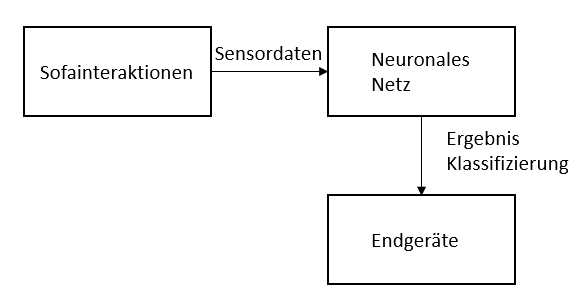
\includegraphics[width=0.6\textwidth]{images/arch_grob.png}
	\caption{Visuelle Darstellung zum Aufbau des Systems}
	\label{fig:arch_grob}
\end{figure}


\section{Architektur des Sofaprototypen aus dem Praxisprojekt}
\label{sec:arch_pp}
Der Prototyp ist ein im Rahmen des Praxisprojekts entwickeltes System, welches als verteilte Architektur aufgebaut ist. Während der Bachelorarbeit wird der Prototyp weiter ausgearbeitet und für die weiteren Versuche so optimiert, wie es in Kapitel \ref{sec:arch_sofa} erläutert ist. In diesem Kapitel wird nur die Version aus dem Praxisprojekt zum Vergleich der aktuellen Version des Prototyps während der Bachelorarbeit erläutert.
\newline
\newline
Ein ESP32 misst die Sensordaten eines Ultrasonic-Sensors sowie eines FSR-Sensors. Zwei Flex-Sensoren sind separat an jeweils einem ESP8266 angeschlossen. So bietet der Prototyp nur die Möglichkeit für eine Person zu sitzen oder auf den Sitzflächen mit den Flex-Sensoren zu liegen. Diese Daten schicken sie an einen Raspberry Pi 2, welcher diese an ein Regelsystem weitergibt, dessen Regeln in \ref{sec:rules} aufgeführt sind. Das Regelsystem ist in dieser Version des Prototypen die Hauptkomponenten, um die Interaktionen zu verwalten. Die verarbeiteten Daten, welche über \emph{if-Abfragen} in Regeln umgewandelt sind, werden über den Broker an die smarten Geräte gesendet. In diesem Prototyp sind noch keine smarten Geräte integriert, da diese Einbindung kein primäres Ziel ist. Mit diesem Prototypen ist es möglich, dass Personen mit festen Interaktionen die smarten Geräte steuern ohne, dass der Nutzer Einfluss auf diesen Vorgang nimmt. Damit sind die Interaktionen davon abhängig, wie der Nutzer mit dem Sofa interagiert. Werden die Sensoren in einer anderen Art und Weise verwendet wie es nicht vom Regelsystem vorgesehen ist, so können die erwünschten smarten Geräte nicht gesteuert werden. Somit ist das Regelsystem ein erheblicher Nachteil für Personen, die das Sofa zum ersten Mal benutzen oder für Personen, welche körperlich oder geistig benachteiligt sind sowie Personen sehr hohen Alters.
\newline
Unter anderem wird aus diesem Grund auch das neuronale Netz entwickelt und ersetzt damit das Regelsystem. Zusätzlich werden die Flex-Sensoren nicht mehr für die Liegepositionen benötigt, da diese nicht dafür geeignet sind. Um die Liegeposition dennoch zu erkennen, übernehmen die Kombinationen der Drucksensoren auf den Sitzkissen diese Aufgabe. Es ist wichtig zu erwähnen, dass die Architektur aus dem Praxisprojekt so ausgelegt ist, dass nur eine Person auf einem Platz sitzen kann und die anderen Sitzkissen nur mit Flex-Sensoren verbaut sind. Auf den nicht besetzten Plätzen ist es jedoch nicht möglich, dass andere Personen dort zusätzlich Platz nehmen. 

\section{Die Anpassung der Architektur für das neuronale Netz}
\label{sec:arch_sofa}
Dieses Kapitel beschreibt die Architektur der Bachelorarbeit und zeigt die Unterschiede aus Kapitel \ref{sec:arch_pp} zur aktuellen Architektur. Kapitel \ref{sec:komm} beschreibt die Kommunikation mit MQTT, weshalb dies auch in diesem Kapitel nicht weiter erläutert wird.

\begin{figure}[H]
	\centering
		%[natürliche Breite in Pixeln, natürliche Höhe in Pixeln, Abhängigkeit von der Textbreite]
		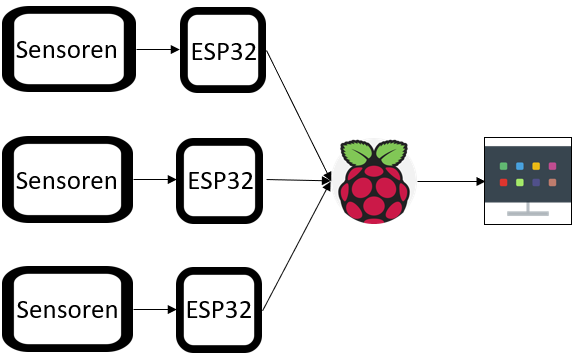
\includegraphics[width=0.6\textwidth]{images/Architektur.png}
	\caption{Abschließende Architektur mit einem Endgerät als Beispiel}
	\label{fig:arch}
\end{figure}

Abbildung \ref{fig:arch} zeigt die Architektur des überarbeiteten Prototypen. Als Sensoren werden Ultrasonic-Sensoren und Force Sensitive Resistores benutzt. Die Ultrasonic-Sensoren messen den Abstand um zu erkennen ob eine Person angelehnt ist. Die FSR-Sensoren messen anhand des Drucks ob eine Person sitzt, liegt oder mit den Armlehnen interagiert. Da dieser Prototyp für ein drei Personen Sofa ausgelegt ist, haben die beiden äußeren ESPs auch jeweils einen FSR für die Armlehnen angeschlossen. Der Raspberry Pi übernimmt die Aufgabe des MQTT-Brokers und der Aufnahme und Weitergabe der Sensorwerte. Der hier dargestellte Fernseher ist ein Beispiel für ein smartes Endgerät. Powerbanks sorgen für die Stromversorgung der Mikrocontroller und des Raspberry Pis. Alternativ ist auch das Anschließen eines Stecker für Steckdosen möglich. Als nächstes ist wichtig zu klären, ob der Prototyp als Cloud-Architektur oder lokales Netzwerk benutzt wird.
\newline
Hinsichtlich dieser Architektur reicht für das System ein lokales Netzwerk aus. Im Vergleich zu einer Cloud-Architektur ist es nicht möglich von außen auf das System zuzugreifen. Da die Steuerung sich nur innerhalb des Smart Homes befindet, reicht das lokale Netzwerk dafür aus. Eine Cloud-Architektur ergibt also nur Sinn, wenn Nutzer außerhalb des im Smart Homes auf die Geräte zugreifen wollen. Das kann der Nutzer aber nicht, da das Sofa sich immer innerhalb des Smart Homes befindet. 

\newpage

\section{Regelsystem zur Steuerung der Interaktionen} 
\label{sec:rules}
Das neuronale Netz ersetzt in der aktuellen Version des Prototypen das Regelsystem. Das Regelsystem ist ein statisches System, welches feste Regeln beinhaltet. Dieses wird in diesem Abschnitt näher erläutert. Es sollen Vor- und Nachteile veranschaulicht werden und weshalb es durch das neuronale Netz ersetzt wird.
\newline
Das Regelsystem ist so ausgelegt, dass je nach Verwendung der Sensoren eine Regel bzw. ein Code erstellt wird. Der Nachteil dieses Systems ist der statische Aufbau. Wenn eine Regel ausgelöst wird, muss jeder Benutzer immer die gleichen Sensoren auslösen um eine Regel zu nutzen. So muss bei einer Erweiterung mit neuen Regeln der Python-Code immer angepasst werden. Das hat den Nachteil für Menschen, die das System nicht kennen und zum ersten Mal benutzen. Vor allem müssen sie den Code selbst erweitern.
\newline
Da sich jede Person anders hinsetzen kann, aber das gleiche Gerät steuern möchte, kann dies nicht vom Regelsystem erkannt werden. Daher hat der Autor die Architektur und damit auch die Weiterführung des Prototypen ersetzt. Die Tabelle \ref{tab:tablerules} beschreibt dennoch noch einmal die Regeln und welche Kombination von Sensoren ausgelöst werden muss, damit man die Regeln an ein smartes Gerät sendet. Die Aufzählungen der Regeln sind auch gleichzeitig die Codes, die gepublished werden, um die smarten Geräte zu steuern. 
\newline
Mit dem Regelsystem gibt es drei FSR-Sensoren und einen Ultrasonic-Sensor für die Sitzpositionen im Prototypen. Für die Liegeposition werden zwei Flex-Sensoren benutzt. Die Flex-Sensoren fallen mit dem einsetzen des neuronalen Netzes weg, da auf den entsprechenden Plätzen andere Sensoren verwendet werden. Dies passiert, weil die Sensoren eine Biegung von mindestens 45 Grad brauchen, damit sie erkennen, dass jemand auf ihnen liegt. Daher werden nun FSR-Sensoren für die Liegepositionen eingebaut. Diese erkennen, ob eine Person sitzt oder liegt. Somit müssen dann nicht mehr zwei Sensoren in die Sitzkissen eingebaut werden. Das positive an diesem Regelsystem ist die Erweiterbarkeit der Regeln für den Entwickler. Dabei wird im Programm nur die neue Regel mit einer \emph{if-Abfrage} erweitert.

\begin{table}[H]
	\centering
	\caption[Aufzählung der Regeln des Regelsystems]{Aufzählung der Regeln des Regelsystems}
		\vspace{1.0em}	
	\begin{tabular}{|l|p{7cm}|}
		\hline
		\rowcolor[gray]{0.9}\textbf{Regeln} & \textbf{Beschreibung} \\
		\hline
		\hline
		1 & Alle FSR-Sensoren und der Ultrasonic-Sensor messen Daten \\
		\hline
		2 & Nur der FSR-Sensor auf dem Sitzkissen misst Daten
		    und der Ultrasonic-Sensor \\
		\hline
		3 & Beide FSR-Sensoren messen Daten \\
		\hline
		4 & Der FSR-Sensor auf dem Sitzkissen misst Daten \\
		\hline
		5 & Der FSR-Sensor auf dem Sitzkissen und die beiden Flex-Sensoren messen Daten \\
		\hline
		6 & Beide Flex-Sensoren messen Sensordaten \\
		\hline
		7 & Ein Flex-Sensor und der FSR-Sensor auf dem Sitzkissen messen Daten \\
		\hline
	\end{tabular}
	\label{tab:tablerules}
\end{table}

\section{Verarbeitung der Daten im ESP und Raspberry Pi}
Kapitel \ref{sec:arch_sofa} zeigt die Verwendung mehrerer ESP32 und einem Raspberry Pi in der Architektur. Die Mikrocontroller und der Einplatinencomputer sind die Hauptkomponenten zur Verarbeitung der Sensordaten. An einem ESP sind mindestens ein FSR-Sensor und maximal ein Ultrasonic-Sensor angeschlossen. Die Sensoren schicken ihre Sensorwerte an den entsprechenden ESP. Die Sensordaten werden als Binary-Werte vom ESP erfasst und an den MQTT-Broker gepublished. Das Python-Programm soll diese Daten auf dem Raspberry Pi als Subscriber empfangen und verarbeiten. Damit das Python-Programm die Sensordaten unterscheiden kann, werden die Sensordaten in einem Array gespeichert. Um unterscheiden zu können, welcher Wert zu welchem Sensor gehört, hat ein Sensor einen eigenen Index in einer Liste. Das Programm wird als Subscriber vom MQTT-Broker erfasst und schickt ihm die Sensorwerte. Die Daten werden in einer CSV-Datei gespeichert. Vorher müssen sie noch encoded werden, damit sie richtig dargestellt werden. Wenn dies nicht passiert, werden die Werte mit dem falschen Datentyp in der CSV-Datei gespeichert. Über eine Funktion aus der MQTT-Bibliothek kann zur besseren Darstellung der Binary-Wert zu Utf-8 encoded werden. Da das neuronale Netz Integer-Werte einliest, muss das Encoding stattfinden, denn die Binary-Werte sind in Python sonst einzelne Char-Datentypen. Dadurch würden die Daten nicht pro Zeile als eine Position gespeichert werden, sondern jeder Wert in einer neuen Zeile. Diese Liste speichert mit den Sensorwerten aktuell noch eine unbekannte Position des Nutzers, da diese Werte noch nicht verarbeitet wurden. Daher werden die Sensorwerte zum trainieren für das neuronale Netz in die CSV-Datei übergeben. 
\newline
Sobald das neuronale Netz die Vorhersagen richtig angibt, besteht die Möglichkeit das Netz in das Python-Programm zu integrieren, welches aber nicht von Vorteil ist wie \ref{sec:einb} zeigt. Zudem wird dann auch nicht mehr jeder Sensorwert in die CSV-Datei übergeben, sondern die Sensorwerte werden einzeln an das neuronale Netz geschickt und dieses versucht die Positionen sofort zu klassifizieren. 

\section{Steuerungsarten eines Smart Homes}
Diese Bachelorarbeit beschäftigt sich mit der Verwaltung von Interaktion zur Steuerung smarter Geräte durch Möbel. Da dies nur eine Möglichkeit zur Steuerung ist, diskutiert der Autor in diesem Kapitel Alternativen zu der Steuerung, welches Thema dieser Bachelorarbeit ist und deren Unterschiede zum aktuell entwickelten Prototypen.
\newline
\newline
Der aktuelle Prototyp, welcher im Praxisprojekt entwickelt wurde und in der Bachelorarbeit weiter entwickelt wird, interagiert passiv mit dem Nutzer. So muss der Nutzer nur seine gewohnten Positionen auf dem Sofa einnehmen und steuert damit die smarten Geräte. Dies spart Zeit, die der Nutzer normalerweise mit einem Tablet oder ähnlichem Gerät beötigen würde um das Smart Home zu steuern. Als weiteren Punkt sollte nicht unerwähnt bleiben, dass mit der Sofasteuerung Nutzungsmöglichkeiten mit den smarten Geräten entfallen. Dies ist ein Nachteil, welcher wiederum durch die zusätzliche Hinzuziehung weiterer Steuerungsmöglichkeiten gelöst werden kann. Das ist jedoch nicht sinnvoll, wenn der Aspekt der Zeitersparnis bestehen bleiben soll. Die folgende wissenschaftliche Arbeit \citep{piyare2013internet} erläutert die Umsetzung einer Steuerung in einem Smart Home über Tablet und Smartphone, welche mit Android umgesetzt wurde.
\newline
Achtet man nicht auf Zeitersparnis und will die individuelle Nutzung der smarten Geräte beibehalten, haben Mobilgeräte und ähnliche Steuerungsgeräte den Vorteil, smarte Geräte in einem breiteren Spektrum zu nutzen. Dafür muss aber entsprechend auch mehr Zeit genutzt werden, da die Geräte oft erst entsperrt werden müssen und unterschiedliche Apps für die smarten Geräte heruntergeladen sein müssen. Also fällt mit dem Nutzen einer Sofasteuerung das Entsperren und die Benutzung verschiedener Apps weg. Zudem sind die Komponenten des Systems an Powerbanks oder direkt an einer Steckdose angeschlossen. So müssen diese Komponenten nicht so oft oder gar nicht wie ein Smartphone oder ähnliches Gerät aufgeladen werden.

\section{Kommunikation der Sensoren mit dem neuronalen Netz}
\label{sec:komm}
Wie in den vorherigen Kapiteln zur Architektur erwähnt, findet die Kommunikation im Prototypen mit MQTT statt. Hier erläutert der Autor dessen Umsetzung und Funktion im Prototypen.
\newline
Um MQTT-Mosquitto auf dem Raspberry Pi zu installieren, müssen dafür bestimmte Commands im Terminal eingegeben werden. Zudem muss die entsprechende Bibliothek in Python installiert werden, damit das Python-Programm mit dem Broker kommunizieren kann. Über 
\newline
\newline
\emph{sudo apt install -y mosquitto mosquitto-clients}
\newline
\newline
wird Mosquitto installiert und daraufhin wird Service mit 
\newline
\newline
\emph{sudo systemctl enable mosquitto.service} aktiviert.
\newline
\newline
Je nach Betriebssystem und dessen Version weichen die Befehle voneinander ab oder es müssen weitere hinzugefügt werden. 
\newline
Ist der Service gestartet, kann darüber kommuniziert werden. Zu Beginn schicken die ESP32 die Sensorwerte mit der Publish-Funktion als eine Byte-Nachricht zum MQTT-Broker. Der MQTT-Broker empfängt die Daten vom Publisher und speichert sie für die Subscriber zwischen. Alle Subscriber empfangen die Daten gleichzeitig und können sie unabhängig voneinander verarbeiten. Wie schon in Kapitel \ref{sec:mqtt} erwähnt, ist es auch möglich, dass die Subscriber die Nachrichten auch empfangen können, wenn die Publisher nicht mit dem MQTT-Broker verbunden sind. Dies ist ein Vorteil, wenn ein Publisher ausfallen sollte, aber der Subscriber die Sensorwerte noch nicht rechtzeitig verarbeiten konnte. Als Subscriber dient in diesem Projekt das Python-Programm, welches diese Daten für das neuronale Netz empfängt. Das Programm befindet sich im ersten Anhang. Bevor das neuronale Netz in den Prototypen eingebunden wird, muss es aber korrekt klassifizieren. Damit das neuronale Netz dies trainieren kann, werden die im Prototyp kommunizierten Daten als CSV-Datei in das neuronale Netz eingelesen. 
\newline
\begin{figure}[H]
	\centering
		%[natürliche Breite in Pixeln, natürliche Höhe in Pixeln, Abhängigkeit von der Textbreite]
		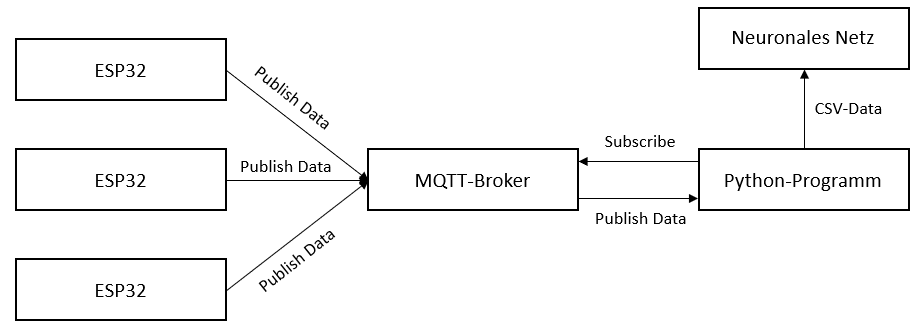
\includegraphics[width=0.9\textwidth]{images/com_arch.png}
	\caption{Die Kommunikationsarchitektur ohne Endgerät als Beispiel}
	\label{fig:com_arch}
\end{figure}
\newline
Das Python-Programm, welches die Daten in einer CSV-Datei speichert, published die Ergebnisse des neuronalen Netzes. Diese Ergebnisse nutzen die smarten Geräte als Steuerung. Abbildung \ref{fig:com_arch} zeigt die Kommunikationsarchitektur ohne die Anbindung an ein smartes Endgerät, da diese Kommunikation noch nicht hergestellt wird. Da die Ergebnisse am Ende gepublished werden, ist die Kommunikation offen, um mit smarten Geräten oder Möbeln zu kommunizieren. Sollte das neuronale Netz weiterhin als eigene Komponenten agieren, so müssen die Ergebnisse auch dementsprechend darüber an den Broker mitgeteilt werden und nicht über das Python-Programm, welches die Sensordaten erfasst. Dies passiert erst, sobald das neuronale Netz vollständig korrekt klassifizieren kann.

\section{Gegenüberstellung eines neuronalen Netzes mit TensorFlow und Numpy}
Um ein neuronales Netz zu programmieren gibt es verschiedene Möglichkeiten. In diesem Kapitel wird die Umsetzung mit der Numpy-Bibliothek und TensorFlow diskutiert. Die entsprechende Umsetzung beider Möglichkeiten findet in Kapitel \ref{sec:ums_nn} statt. Da in dieser Arbeit beide Möglichkeiten umgesetzt wurden, befinden sich auch entsprechend beide Erläuterungen im genannten Kapitel.
\newline
\newline
Da Numpy schon eine integrierte Standardbibliothek in Python ist, muss man sich keine weiteren Gedanken machen, eine externe Bibliothek in Python einzubinden. Der Aufbau eines neuronalen Netzes mit dieser Bibliothek muss komplett selbst gestaltet und entwickelt werden. So müssen also Aktivitätsfunktionen, Feedforward- und Backpropagation-Schritte erstellt werden, welche nicht aus der Bibliothek wie in TensorFlow bzw. Keras zur komfortableren Entwicklung mit entsprechenden Funktionen schon enthalten sind. Daher besteht der Vorteil mit TensorFlow unterschiedliche Kombinationen für ein neuronales Netz schneller Umsetzen und Ausprobieren zu können.
\newline
Wird bei der Entwicklung nur Numpy verwendet, lässt sich die sigmoid-Funktion zum Beispiel einfach Umsetzen, da Numpy eine mathematische Bibliothek von Python ist. Anders als mit Keras, bei der im entsprechenden Layer einfach der Name der Aktivitätsfunktion angegeben werden kann. Durch die mathematischen Vorteile mit Numpy kann ein einfaches neuronales Netz sehr simpel aufgebaut werden. Durch die einfache Umsetzung eines simplen neuronalen Netzes mit Numpy hat sich der Autor zu Beginn erst dafür entschieden, weil TensorFlow zu Beginn der Bachelorarbeit zu mächtig für kleine neuronale Netze ist und Keras dafür dem Autor nicht bekannt war. Weiterhin ist bei der Einschätzung aufgefallen, dass TensorFlow eher für Deep Neural Networks geeignet ist. Also für neuronale Netze mit mehr als zwei Hidden-Layer. Da das neuronale Netz nicht die gewünschten Ergebnisse liefert und zu einfach für die Anforderungen gestaltet ist, ist ein Umstieg auf die Einbindung von Keras als Frontend-Engine mit TensorFlow als Backend-Engine von Vorteil. Durch den Umstieg ist es möglich, einfach Layer hinzuzufügen und besser entscheiden zu können, welche Daten aus den Datensätzen für das Training und für den Test benutzt werden. Um einfach kleinere Netze zu programmieren reicht es aus, Numpy für die Umsetzung zu verwenden und Keras für Netze, die größer sind.

\section{Zusammenfassung und Ausblick}
Mit der beschriebenen Architektur zum Prototypen und dem neuronalen Netz möchte der Autor zeigen, dass es möglich ist, die Anforderungen und das Ziel aus Kapitel \ref{sec:goal} zum Prototypen umzusetzen. Des weiteren besteht damit die Möglichkeit dieses Gesamtsystem über den Prototypen hinaus weiterzuentwickeln, um diesen als finale Steuerung in ein Smart Home einzubinden. 
\newline
Die Gegenüberstellung der Architektur aus dem Praxisprojekt zum System in der Bachelorarbeit, zeigt, dass es besser ist einen Prototypen zu verwenden, welcher eine Komponente pro Sitzplatz auf dem Sofa verwendet. So ist es möglich, ein Sofa als Steuerung in größerem Umfang zu nutzen, wenn z.B. die Steuerung abhängig von der Sitzplatzzahl auf dem Sofa ist. Zusätzlich ist es mit dem Prototyp auch möglich, dass mehrere Personen gleichzeitig auf dem Sofa sitzen können und dies als Klassifizierung hinzu genommen werden kann. Dies wird allerdings nicht vom neuronalen Netz in dieser Arbeit mit einbezogen. Das zeigt die Möglichkeiten, welche in Zukunft implementiert werden können. So ist es wichtig, dass die Sensoren nicht beim Einbau in einem Sofa auffallen. Die Anzahl oder Größe der Sensoren spielt auch eine Rolle, damit der Nutzer das Sofa in vollem Umfang zur Steuerung benutzen kann. Daher sollte bei der Auswahl der Sensoren die Größe der jeweils zu messenden Fläche beachtet werden.
\newline
Beim neuronalen Netz ist es von Vorteil bei größeren Umsetzungen auf Bibliotheken wie TensorFlow zurückzugreifen. Für einfache Netze reicht Numpy aus, da man dort individuell ohne Bindung an Funktionen, die nicht unbedingt die gewünschten Ergebnisse bringen, die Umsetzung realisieren kann.
\newline
Wenn TensorFlow und Keras genutzt wird, können sehr einfach und schnell große neuronale Netze realisiert werden. Dies zeigt auch \citep{frochte2018} bei der Umsetzung eines neuronalen Netzes mit Keras und TensorFlow. In Zukunft ist es wichtig, dass die Sensoren weiter angepasst werden. Zusätzliche Klassifizierungen erweitern dann auch die Interaktionsmöglichkeiten mit dem Sofaprototypen.